\maketitlesupplementary
\appendix
\setcounter{page}{1}
\setcounter{table}{0}
\setcounter{figure}{0}
\setcounter{equation}{0}
\counterwithin{figure}{section}
\counterwithin{table}{section}
\renewcommand{\thetable}{\thesection.\arabic{table}}
\renewcommand{\thefigure}{\thesection.\arabic{figure}}
\renewcommand{\theequation}{\thesection.\arabic{equation}}


\section{Depth Estimation Analysis}
\label{app:depth-analysis}
\paragraph{Robustness to depth quality.}
Our method is designed to be tolerant of moderate noise in estimated depth. As shown in \cref{fig:depth-noise-ablation-v4}, tracking performance remains stable under additive Gaussian noise up to $\sigma$ = 2\,cm. This robustness stems from extensive training augmentations and from the transformer’s ability to interpolate and re-identify points even when partial depth information is missing or corrupted. 

\paragraph{Depth source comparisons.}
\cref{tab:depth-types} summarizes performance across different depth sources, including sensor depth, optimization-based reconstruction, and learned estimators (DUSt3R and VGGT). Our method achieves strong performance with noisy but plausible depth maps from learned estimators, particularly VGGT, but degrades significantly when depth estimation produces misaligned geometry or fails.

\paragraph{DUSt3R alignment and runtime.}
To align DUSt3R~\cite{wang2024dust3r} reconstructions to our camera setup, we globally optimize the pairwise maps using its built-in alignment (following Sec.~3.4 in DUSt3R), while keeping our camera intrinsics and extrinsics fixed. This reconstruction step takes 300 iterations and runs at 0.17 FPS. VGGT offers a significantly faster alternative at 3.1 FPS.

\paragraph{Discussion.}
Sparse-view reconstruction remains an open problem. In our evaluations, DUSt3R was the most reliable method for producing usable depth maps, but even it fails on some scenes. As depth estimation continues to improve, particularly with recent advances in foundation models for geometry (e.g., MegaSAM~\cite{li2024_megasam}, Easi3R~\cite{chen2025easi3r}), MVTracker can directly benefit (with or without retraining). \cref{fig:depths} visualizes our predicted tracks under different depth sources, and \cref{tab:depth-types} quantifies performance across depth sources.

\begin{table}[h]
\centering
\caption{\textbf{AJ for different depth sources.} GT*: optimization-based depth. D: DUSt3R. V: VGGT. S: Sensor. \ding{55}: depth estimation failed.}
\vspace{-0.35cm}
\resizebox{\columnwidth}{!}{%
\begin{tabular}{l ccc ccc ccc}
\toprule
\multirow{2}{*}{Method}
& \multicolumn{3}{c}{Panoptic Studio}
& \multicolumn{3}{c}{DexYCB}
& \multicolumn{3}{c}{MV-Kubric}
\\
\cmidrule(lr){2-4} \cmidrule(lr){5-7} \cmidrule(lr){8-10}
& GT* & D & V & S & D & V & GT & D & V \\
\midrule
DELTA              &    68.1  & \ding{55} &     1.8  &    54.6  &    36.8  &    21.1  &    57.4  &    25.7  &     1.9  \\
SpaTracker         &    61.5  & \ding{55} &    10.6  &    60.9  &    58.3  &    33.2  &    65.5  &    61.7  &     3.9  \\
Triplane Baseline  &    65.1  & \ding{55} &    29.7  &    68.0  &    57.5  &    61.8  &    74.7  & \B{70.7} &    46.7  \\ \rowcolor{cyan!16}
MVTracker (ours)   & \B{86.0} & \ding{55} & \B{47.7} & \B{82.7} & \B{71.6} & \B{68.0} & \B{81.4} &    70.0  & \B{48.7} \\
\bottomrule
\end{tabular}
}
\label{tab:depth-types}
\end{table}

\begin{figure}[h]
    \centering
    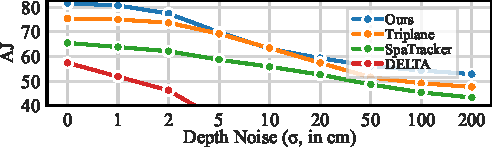
\includegraphics[width=\linewidth]{figures/plot_robustness_to_depth_noise.pdf}
    \vspace{-0.7cm}
    \caption{
    \textbf{Robustness to depth noise $\mathcal{N}(0, \sigma^2)$ on MV-Kubric.}}
    \label{fig:depth-noise-ablation-v4}
\end{figure}

\begin{figure}[h]
    \centering  
    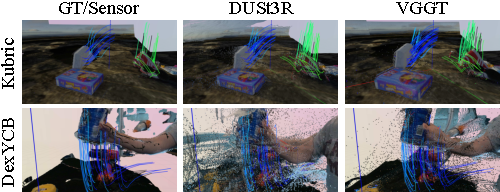
\includegraphics[width=\linewidth]{figures/depth-sources.pdf}
    \vspace{-0.7cm}
    \caption{\textbf{Different depth sources along our predicted tracks.}}
    \label{fig:depths}
\end{figure}


\section{Inference Speed Comparison}
\label{app:sec:inference}

We evaluate the runtime of various methods by measuring frames per second (FPS) on a representative test configuration. \cref{tab:fps_comparison} summarizes the results, excluding depth-estimation time. For \emph{optimization-based} methods such as Shape of Motion~\cite{som2024} and Dynamic 3D Gaussians~\cite{luiten2023dynamic}, the per-sequence runtime is significantly higher (\eg, about 30 minutes for Shape of Motion and about 50 minutes for Dynamic 3DGS on a single Panoptic Studio~\cite{koppula2024tapvid} sequence). Overall, the optimization-based approaches are orders of magnitude slower, making them less practical for large-scale applications and unusable for real-time applications. In contrast, our feed-forward model runs online at a comparable speed to the triplane-based baseline while outperforming it in accuracy, highlighting the efficiency of our kNN correlation in 3D point clouds. Note that we correctly adjust the effective FPS by taking into account the window size for sliding-window-based methods.

\begin{table}[h]
\setlength{\tabcolsep}{2pt}
\centering
\caption{\textbf{Runtime Comparison (FPS).} We measure frames per second for each method under a representative test setting, excluding depth-estimation overhead. Optimization-based methods are indicated with placeholders for their much lower throughput.}
\vspace{-0.3cm}
\begin{tabular}{l c}
\toprule
\textbf{Method} & \textbf{FPS} \\
\midrule
Dynamic 3DGS~\cite{luiten2023dynamic}     & \emph{(optimization-based)} \\
Shape of Motion~\cite{som2024}            & \emph{(optimization-based)} \\
SpaTracker~\cite{xiao2024spatialtracker} &  1.4 \\
DELTA~\cite{ngo2024delta}                &  1.5 \\
SceneTracker~\cite{wang2024scenetracker} &  3.5 \\ %
CoTracker2~\cite{karaev2023cotracker}    &  5.7 \\
Triplane Baseline                        &  5.8 \\
\rowcolor{cyan!16}MVTracker (ours)      &  7.2 \\ %
CoTracker3~\cite{karaev24cotracker3}     & 18.4\\
\bottomrule
\end{tabular}
\label{tab:fps_comparison}
\end{table}





\section{Ablation Study} \label{app:sub:ablation}

\subsection{Impact of Different Depth Sources}
\Cref{tab:dexycb-depth-types} reports the performance of our model and several baselines on DexYCB when using two different depth sources: DUSt3R~\cite{wang2024dust3r} (estimated) and sensor-based depth. We observe that sensor-based depth leads to improved accuracy for all methods, highlighting the importance of depth quality. Notably, our multi-view tracker benefits substantially from sensor depth, surpassing single-view methods and the triplane baseline by a larger margin. This suggests that our fused 3D point cloud representation is robust to a wide range of depth sources, yet can further leverage higher-fidelity depth to achieve stronger 3D point tracking.
\begin{table}
\setlength{\tabcolsep}{2pt}
\centering
\caption{\textbf{Impact of Different Depth Sources} on DexYCB. We report results using either DUSt3R-estimated~\cite{wang2024dust3r} or sensor-based depth for all methods. Sensor depth generally improves performance across the board, underscoring the importance of high-fidelity depth. Notably, our multi-view tracker benefits the most, indicating that our fused 3D point cloud representation effectively capitalizes on better depth quality.
}
\vspace{-0.3cm}
\begin{tabular}{l cccc}
                  \toprule
                                    Method &   AJ\hspace{-0.01cm}\ua & \davg\hspace{-0.05cm}\ua &   OA\hspace{-0.03cm}\ua\hspace{0.03cm} &  \hspace{-0.1cm}MTE\hspace{-0.03cm}\da \\
                  \midrule
                \multicolumn{5}{r}{DexYCB~\cite{dexycb} (DUSt3R depth) } \\
\midrule
LocoTrack~\cite{cho2024local}                &    27.8  &    38.6  &    77.0  &    22.8  \\ 
DELTA~\cite{ngo2024delta}                    &    36.8  &    51.6  &    61.0  &    18.3  \\ 
CoTracker2~\cite{karaev2023cotracker}        &    28.8  &    40.5  &    76.2  &    20.8  \\ 
CoTracker3~\cite{karaev24cotracker3}         &    29.4  &    40.3  &    78.6  &    22.0  \\ 
SpaTracker~\cite{xiao2024spatialtracker}     &    58.3  &    72.0  &    80.2  &     5.9  \\ 
SpaTrackerV2~\cite{xiao2025spatialtrackerv2} &    35.5  &    45.1  &    91.3  &     9.8  \\
TAPIP3D~\cite{tapip3d}                       &    38.8  &    50.0  &    90.1  &     8.2  \\
Triplane Baseline                            &    57.5  &    71.0  &    81.3  &     4.3  \\ 
\rowcolor{cyan!16} MVTracker (ours)          & \B{71.6} & \B{80.6} & \B{91.3} &  \B{2.0} \\ 


                  \toprule
                 \multicolumn{5}{r}{DexYCB~\cite{dexycb} (sensor depth)} \\
                  \toprule
LocoTrack~\cite{cho2024local}                &    55.1  &    64.6  &    76.7  &    27.5  \\
DELTA~\cite{ngo2024delta}                    &    54.6  &    67.8  &    72.6  &    42.6  \\
CoTracker2~\cite{karaev2023cotracker}        &    56.4  &    67.4  &    76.4  &    26.4  \\
CoTracker3~\cite{karaev24cotracker3}         &    57.3  &    68.5  &    76.7  &    23.4  \\
SpaTracker~\cite{xiao2024spatialtracker}     &    60.9  &    75.0  &    82.5  &     4.0  \\
SpaTrackerV2~\cite{xiao2025spatialtrackerv2} &    69.2  &    77.5  &    91.3  &     4.2  \\
TAPIP3D~\cite{tapip3d}                       &    77.2  &    88.9  &    88.0  &     1.3  \\
Triplane Baseline                            &    68.0  &    79.5  &    85.9  &     2.6  \\
\rowcolor{cyan!16} MVTracker (ours)          & \B{82.7} & \B{91.0} & \B{91.6} &  \B{0.8} \\
\bottomrule
\end{tabular}
\label{tab:dexycb-depth-types}
\end{table}



\subsection{Varying the Number of Input Views}
\label{sec:number-of-views-details}
\cref{tab:ablate-number-of-views} shows detailed per-dataset results for a varied number of input views. Our tracker consistently improves as more views are added.

\begin{table}[t]
\setlength{\tabcolsep}{1.2pt}
\centering
\caption{\textbf{Varying the Number of Input Views.} Evaluation of AJ under a varied number of input views.}
\vspace{-0.3cm}
\begin{tabular}{lcccccccc}
                                             \toprule \multirow{2}{*}[0.07em]{Method} & \multicolumn{8}{c}{Number of views} \\
                                             &       1  &       2  &       3  &        4 &       5  &       6  &       7  &       8  \\
                                             \toprule
                                             & \multicolumn{8}{c}{Panoptic Studio~\cite{koppula2024tapvid}} \\
                                             \toprule
LocoTrack~\cite{cho2024local}                &     54.7 &    56.4  &    61.4  &    65.8  &    65.8  &    67.3  &    66.4  &    66.8  \\
DELTA~\cite{ngo2024delta}                    &     60.9 &    61.8  &    63.7  &    68.1  &    66.7  &    67.4  &    67.6  &    66.3  \\
CoTracker2~\cite{karaev2023cotracker}        &     59.5 &    60.7  &    64.4  &    69.5  &    68.8  &    69.3  &    68.4  &    69.9  \\
CoTracker3~\cite{karaev24cotracker3}         &     61.9 &    65.0  &    68.5  &    74.5  &    74.0  &    75.2  &    75.1  &    76.0  \\
SpaTracker~\cite{xiao2024spatialtracker}     &     51.2 &    52.1  &    57.5  &    61.5  &    60.9  &    61.4  &    62.6  &    63.4  \\
SpaTrackerV2~\cite{xiao2025spatialtrackerv2} &     57.4 &    62.7  &    66.8  &    72.4  &    71.8  &    72.7  &    72.7  &    72.9  \\
TAPIP3D~\cite{tapip3d}                       &  \B{68.8}& \B{72.9} &    78.5  &    84.3  &    84.6  &    85.6  &    86.0  &    86.8  \\
Triplane Baseline                            &     61.9 &    60.9  &    61.6  &    65.0  &    64.0  &    65.1  &    66.8  &    65.6  \\
\rowcolor{cyan!16} MVTracker (ours)          &    66.4  &    72.2  & \B{79.0} & \B{86.0} & \B{87.4} & \B{88.8} & \B{89.1} & \B{89.9} \\
                                             \toprule
                                             & \multicolumn{8}{c}{DexYCB~\cite{dexycb} (DUSt3R depth)} \\
                                             \toprule
LocoTrack~\cite{cho2024local}                &     27.9 &    26.0  &    28.1  &    27.8  &    36.3  &    34.8  &    34.7  &    34.9  \\
DELTA~\cite{ngo2024delta}                    &     33.0 &    34.3  &    38.0  &    36.5  &    37.2  &    35.4  &    34.9  &    35.7  \\
CoTracker2~\cite{karaev2023cotracker}        &     29.8 &    26.4  &    29.2  &    28.8  &    37.8  &    36.2  &    36.0  &    36.0  \\
CoTracker3~\cite{karaev24cotracker3}         &     28.6 &    27.0  &    29.5  &    29.4  &    39.1  &    37.5  &    37.1  &    37.3  \\
SpaTracker~\cite{xiao2024spatialtracker}     &     60.6 &    58.4  &    61.8  &    58.3  &    63.2  &    62.4  &    62.9  &    63.4  \\
SpaTrackerV2~\cite{xiao2025spatialtrackerv2} &     39.8 &    39.5  &    36.5  &    35.5  &    41.1  &    37.1  &    37.0  &    37.7  \\
TAPIP3D~\cite{tapip3d}                       &     36.6 &    35.6  &    40.5  &    38.8  &    57.7  &    54.2  &    55.2  &    56.4  \\
Triplane Baseline                            &     44.0 &    48.0  &    56.0  &    57.6  &    63.5  &    64.5  &    65.5  &    66.8  \\
\rowcolor{cyan!16} MVTracker (ours)          & \B{64.0} & \B{66.8} & \B{73.2} & \B{71.1} & \B{77.4} & \B{76.7} & \B{77.3} & \B{79.2} \\
                                             \toprule
                                             & \multicolumn{8}{c}{Multi-View Kubric~\cite{greff2022kubric}} \\
                                             \toprule
LocoTrack~\cite{cho2024local}                &    57.3  &    56.1  &    53.8  &    52.5  &    52.3  &    52.1  &    51.6  &    51.8  \\
DELTA~\cite{ngo2024delta}                    &    65.9  &    61.9  &    58.9  &    57.4  &    56.3  &    56.0  &    54.8  &    54.1  \\
CoTracker2~\cite{karaev2023cotracker}        &    61.4  &    59.1  &    56.1  &    54.6  &    53.8  &    53.7  &    53.1  &    52.8  \\
CoTracker3~\cite{karaev24cotracker3}         &    60.1  &    58.7  &    56.5  &    55.1  &    54.8  &    54.6  &    54.2  &    54.3  \\
SpaTracker~\cite{xiao2024spatialtracker}     &    72.8  &    70.3  &    67.4  &    65.5  &    64.8  &    64.5  &    63.1  &    62.7  \\
SpaTrackerV2~\cite{xiao2025spatialtrackerv2} &     54.0 &    57.6  &    57.6  &    58.6  &    58.3  &    59.1  &    58.8  &    59.7  \\
TAPIP3D~\cite{tapip3d}                       &     76.4 &    75.4  &    72.8  &    72.5  &    71.7  &    71.4  &    70.9  &    70.6  \\
Triplane Baseline                            &    71.7  &    73.4  &    74.1  &    74.7  &    75.0  &    75.2  &    75.2  &    75.7  \\
\rowcolor{cyan!16} MVTracker (ours)          & \B{81.7} & \B{81.2} & \B{81.4} & \B{81.4} & \B{81.9} & \B{82.1} & \B{82.3} & \B{82.5} \\
\bottomrule
\end{tabular}
\label{tab:ablate-number-of-views}
\end{table}


\subsection{2D Tracking Accuracy} 
\begin{table}
\setlength{\tabcolsep}{2pt}
\centering
\caption{\textbf{2D Tracking Evaluation.} Evaluation of projected 2D tracking performance using standard 2D metrics~\cite{doersch2023tapvid}. Multi-view outputs are projected onto four views and the metrics are averaged across these views. Note that we can only report location accuracies since our multi-view methods report any-view visibility (not per-view).}
\vspace{-0.3cm}
\begin{tabular}{lcccccccc}
                                             \toprule {Method}
                                             &       $\delta_\text{avg}^{\text{2D}}$\ua
                                             &       $\delta_{< 1}^{\text{2D}}$\ua
                                             &       $\delta_{< 2}^{\text{2D}}$\ua
                                             &       $\delta_{< 4}^{\text{2D}}$\ua
                                             &       $\delta_{< 8}^{\text{2D}}$\ua
                                             &       $\delta_{<16}^{\text{2D}}$\ua
                                             \vspace{0.05cm}
                                             \\
                                             \toprule
                                             & \multicolumn{6}{c}{Panoptic Studio~\cite{koppula2024tapvid}} \\
                                             \toprule
LocoTrack~\cite{cho2024local}                &    66.7  &    29.3  &    51.4  &    72.6  &    86.5  &    93.7  \\
DELTA~\cite{ngo2024delta}                    &    70.0  & \B{34.8} &    56.5  &    76.5  &    87.6  &    94.8  \\
CoTracker2~\cite{karaev2023cotracker}        &    64.3  &    28.0  &    49.3  &    69.7  &    82.9  &    91.4  \\
CoTracker3~\cite{karaev24cotracker3}         &    70.9  &    33.1  & \B{56.8} &    78.2  &    90.5  &    96.2  \\
SpaTracker~\cite{xiao2024spatialtracker}     &    66.4  &    29.3  &    51.8  &    71.8  &    85.7  &    93.3  \\
Triplane Baseline                            &    51.9  &     8.5  &    24.1  &    52.0  &    80.3  &    94.5  \\
\rowcolor{cyan!16} MVTracker (ours)         & \B{70.5} &    26.6  &    52.9  & \B{79.5} & \B{94.6} & \B{98.9} \\
                                             \toprule
                                             & \multicolumn{6}{c}{DexYCB~\cite{dexycb} (sensor depth)} \\
                                             \toprule
LocoTrack~\cite{cho2024local}                &    83.7  &    74.1  &    78.4  &    84.0  &    89.4  &    92.4  \\
DELTA~\cite{ngo2024delta}                    &    84.6  &    75.7  &    79.9  &    85.2  &    89.4  &    92.8  \\
CoTracker2~\cite{karaev2023cotracker}        &    83.7  &    73.7  &    78.9  &    84.5  &    89.3  &    92.1  \\
CoTracker3~\cite{karaev24cotracker3}         &    84.1  &    74.8  &    79.0  &    84.5  &    89.4  &    92.9  \\
SpaTracker~\cite{xiao2024spatialtracker}     &    85.8  & \B{75.9} &    80.7  &    86.1  &    91.2  &    94.9  \\
Triplane Baseline                            &    75.9  &    52.2  &    70.4  &    78.9  &    85.9  &    92.0  \\
\rowcolor{cyan!16} MVTracker (ours)         & \B{87.5} &    73.3  & \B{81.2} & \B{88.3} & \B{95.5} & \B{99.2} \\
                                             \toprule
                                             & \multicolumn{6}{c}{Multi-View Kubric~\cite{greff2022kubric}} \\
                                             \toprule
LocoTrack~\cite{cho2024local}                &    75.3  &    53.6  &    66.8  &    78.0  &    86.1  &    91.9  \\
DELTA~\cite{ngo2024delta}                    &    78.4  &    61.9  &    72.0  &    80.3  &    86.5  &    91.2  \\
CoTracker2~\cite{karaev2023cotracker}        &    72.6  &    51.8  &    63.7  &    74.2  &    83.1  &    90.2  \\
CoTracker3~\cite{karaev24cotracker3}         &    74.8  &    54.2  &    66.3  &    76.8  &    85.4  &    91.5  \\
SpaTracker~\cite{xiao2024spatialtracker}     &    75.8  &    51.4  &    65.8  &    79.3  &    88.5  &    94.0  \\
Triplane Baseline                            &    80.6  &    51.3  &    72.4  &    87.3  &    94.5  &    97.7  \\
\rowcolor{cyan!16} MVTracker (ours)         & \B{86.8} & \B{61.2} & \B{81.7} & \B{94.0} & \B{97.9} & \B{99.2} \\
\bottomrule
\end{tabular}
\label{tab:ablate-per-view-2d-point-tracking-performance}
\end{table}


\cref{tab:ablate-per-view-2d-point-tracking-performance} compares the performance of 2D point tracking methods when their outputs are projected into 2D using standard metrics~\cite{doersch2023tapvid}. Although 2D methods do not rely on estimated depth quality, they generally achieve lower location accuracies compared to our multi-view approach, which fuses multi-view data to enhance performance. On DexYCB, we only report results using sensor depth maps to provide a more informative comparison in 2D point tracking. For results with depth estimated by DUSt3R, where single-view methods benefit from not having to handle noisy or incomplete depth maps, see \cref{tab:ablate-per-view-2d-point-tracking-performance-dexycb}. Note that such depth noise or incompleteness affects our 2D tracking more than that of SpaTracker, due to SpaTracker’s XY-aligned feature plane compared to our fused 3D point cloud.

\begin{table}
\setlength{\tabcolsep}{2pt}
\centering
\caption{Evaluation of projected 2D tracking performance using standard 2D metrics~\cite{doersch2023tapvid} on DexYCB with estimated depths. Single-view methods only require RGB for tracking and do not depend on the quality of the depth for achieving high 2D point tracking performance. However, the multi-view methods face challenges when dealing with the noisy depth estimates on DexYCB.}
\vspace{-0.3cm}
\begin{tabular}{lcccccccc}
                                             \toprule {Method}
                                             &       $\delta_\text{avg}^{\text{2D}}$\ua
                                             &       $\delta_{< 1}^{\text{2D}}$\ua
                                             &       $\delta_{< 2}^{\text{2D}}$\ua
                                             &       $\delta_{< 4}^{\text{2D}}$\ua
                                             &       $\delta_{< 8}^{\text{2D}}$\ua
                                             &       $\delta_{<16}^{\text{2D}}$\ua
                                             \vspace{0.05cm}
                                             \\
                                             \toprule
                                             & \multicolumn{6}{c}{DexYCB~\cite{dexycb} (DUSt3R depth)} \\
                                             \toprule
LocoTrack~\cite{cho2024local}                &    85.4  &    75.6  &    80.0  &    85.8  &    91.4  &    94.4  \\
DELTA~\cite{ngo2024delta}                    &    85.6  & \B{77.0} &    81.2  &    86.0  &    90.2  &    93.7  \\
CoTracker2~\cite{karaev2023cotracker}        &    86.2  &    75.7  &    81.3  &    87.1  &    92.1  &    95.0  \\
CoTracker3~\cite{karaev24cotracker3}         & \B{86.7}  & \B{77.0} & \B{81.5} & \B{87.2} & \B{92.1} & \B{95.7} \\
SpaTracker~\cite{xiao2024spatialtracker}     &    86.0  &    76.4  &    80.8  &    86.2  &    91.7  &    95.1  \\
Triplane Baseline                            &    64.3  &    31.8  &    53.6  &    71.4  &    79.3  &    85.4  \\
\rowcolor{cyan!16} MVTracker (ours)          &    71.3  &    42.1  &    59.8  &    76.0  &    85.2  &    93.5  \\
\bottomrule
\end{tabular}
\label{tab:ablate-per-view-2d-point-tracking-performance-dexycb}
\end{table}

\subsection{Training Augmentation} \label{app:sec:trainingdetails}
\begin{table}
\setlength{\tabcolsep}{2pt}
\centering
\caption{\textbf{Training Augmentation} of the variable number of input views ranging from 1 to 8  (V) and varying depth sources between ground-truth and off-the-shelf depth estimation (D) during training on tracking performance.} 
\vspace{-0.3cm}
\begin{tabular}{cc c cccc}
\toprule
V & D                 &&   AJ \ua & \davg\ua &   OA \ua &  MTE \da \\
                      \toprule
                      &&& \multicolumn{4}{c}{Panoptic Studio~\cite{koppula2024tapvid}} \\
                      \toprule
\ding{51} &           &&    80.4  & \B{94.4} &    87.8  &  \B{3.1 }\\
          & \ding{51} && \B{80.7} &    93.3  & \B{88.7} &     3.5  \\\rowcolor{cyan!16}
\ding{51} & \ding{51} && \B{80.7} &    94.3  &    88.2  &     3.2  \\
                      \toprule
                      &&& \multicolumn{4}{c}{DexYCB~\cite{dexycb}} \\
                      \toprule
\ding{51} &           &&    49.9  &    72.4  &    70.5  &     3.6  \\
          & \ding{51} &&    62.3  &    77.1  &    82.1  &     3.2  \\\rowcolor{cyan!16}
\ding{51} & \ding{51} && \B{65.2} & \B{79.5} & \B{82.9} &  \B{2.3 }\\
                      \toprule
                      &&& \multicolumn{4}{c}{Multi-View Kubric~\cite{greff2022kubric}} \\
                      \toprule
\ding{51} &           &&    80.2  & \B{91.1}  &    91.1  &  \B{0.7 }\\
          & \ding{51} &&    77.2  &    88.0  &    91.0  &     0.8  \\\rowcolor{cyan!16}
\ding{51} & \ding{51} && \B{80.4} &    90.5  & \B{92.1} &  \B{0.7 }\\
\bottomrule
\end{tabular}
\label{tab:ablate-augmentation-for-main-4view-result}
\end{table}


\begin{table}
\setlength{\tabcolsep}{2pt}
\centering
\caption{\textbf{Training Augmentation} with evaluation on different numbers of views. We investigate the impact of using a variable number of views ranging from 1 to 8 (V) and varying depth sources between ground-truth and off-the-shelf depth estimation (D) during training on tracking performance. Results are reported in AJ.}
\vspace{-0.3cm}
\begin{tabular}{cccccccccc}
\toprule
\multirow{2}{*}[0.1em]{V} & \multirow{2}{*}[0.1em]{D} 
                      & \multicolumn{8}{c}{Number of views} \\
          &           &       1  &       2  &       3  &        4 &       5  &       6  &       7  &       8  \\
                      \toprule
                      && \multicolumn{8}{c}{Panoptic Studio~\cite{koppula2024tapvid}} \\
                      \toprule
\ding{51} &           & \B{69.3} &    72.0  &    76.9  &    80.4  &    81.4  & \B{84.4} &    84.8  &    85.1  \\
          & \ding{51} &    67.0  &    71.3  & \B{77.2} & \B{80.7} & \B{81.9} &    84.2  & \B{84.9} & \B{85.8} \\\rowcolor{cyan!16}
\ding{51} & \ding{51} &    68.1  & \B{73.1} &    76.9  & \B{80.7} &    81.5  &    83.4  &    84.4  &    84.3  \\
                      \toprule
                      && \multicolumn{8}{c}{DexYCB~\cite{dexycb} (DUSt3R depth)} \\
                      \toprule
\ding{51} &           &    37.6  &    40.0  &    48.1  &    49.9  &    65.6  &    67.4  &    69.6  &    73.4  \\
          & \ding{51} &    51.6  &    54.1  &    60.7  &    62.3  &    68.8  &    69.9  &    71.8  &    74.8  \\\rowcolor{cyan!16}
\ding{51} & \ding{51} & \B{56.3} & \B{58.9} & \B{64.9} & \B{65.2} & \B{74.0} & \B{75.4} & \B{76.3} & \B{78.9} \\
                      \toprule
                      && \multicolumn{8}{c}{Multi-View Kubric~\cite{greff2022kubric}} \\
                      \toprule
\ding{51} &           & \B{80.7} & \B{79.9} & \B{80.1} &    80.2  &    80.9  &    81.4  & \B{81.8} &    81.9  \\
          & \ding{51} &    75.9  &    76.3  &    76.6  &    77.2  &    77.2  &    78.0  &    78.1  &    78.4  \\\rowcolor{cyan!16}
\ding{51} & \ding{51} &    80.4  &    79.6  & \B{80.0} & \B{80.4} & \B{81.1} & \B{81.6} & \B{81.8} & \B{82.0} \\
\bottomrule
\end{tabular}
\label{tab:ablate-augmentation-for-varying-views}
\end{table}


\cref{tab:ablate-augmentation-for-main-4view-result} and~\ref{tab:ablate-augmentation-for-varying-views} evaluate the impact of training augmentation strategies. We consider two factors: (V) employing a variable number of views during training (ranging from 1 to 8) and (D) varying the source of depth maps (ground-truth versus off-the-shelf depth estimation). The results reveal that combining both variable view and depth augmentations leads to the best performance, especially as measured on DexYCB.

We apply a range of augmentations to improve generalization and robustness. These include photometric augmentations such as color jitter, Gaussian blur, and occlusion simulation via erasing and region replacement. Spatial augmentations involve random cropping, padding, flipping, and scaling. Depth perturbations include noise, rescaling, and occlusion-based erasure. Scene-level augmentations transform the world coordinate system through random rotation, translation, and scaling. Camera intrinsics and extrinsics are perturbed to simulate realistic variations. Additionally, we vary the number of tracks per sample, randomly sample the number of input views (between 1 and 6), and use either ground-truth depths or depths from an estimation method to improve model adaptability. 

\section{Baselines}
\label{app:sec:baseline_implementation}
\textbf{Dynamic 3D Gaussians.} We use the original training code provided by the authors of the Dynamic 3D Gaussians \cite{luiten2023dynamic}. The training process utilizes camera intrinsics, extrinsics, segmentation masks, images, and an initial point cloud. This initial point cloud is constructed from depth maps corresponding to selected viewpoints at the initial timestep. To differentiate between static and dynamic points within the point cloud, we leverage the provided segmentation masks.

For tracking, we identify the most influential Gaussian for a given point at time $t$ based on the influence computation described in the Dynamic 3DGS paper. To establish a trajectory, we then track the motion of this Gaussian across all time steps. The visibility of each point at time $t$ is determined by comparing the depth of the Gaussian with the corresponding depth value of the depth map rendered from each camera viewpoint. Trajectories that show sudden discontinuities or have a dominant Gaussian influence near zero for the query point are classified as static to ensure consistency in motion.

To evaluate the model's performance in novel view synthesis, we conducted experiments on Panoptic Studio. We trained different models using a varying number of cameras. Then, we render images using these trained models from four test cameras. Our results in \cref{tab:d3dgs-vary-number-of-views} show that with 27 input views, we achieve reconstruction quality comparable to that reported in the original paper. However, as the number of views decreases, reconstruction quality reduces.
\begin{table}[t]
\setlength{\tabcolsep}{4pt}
\centering
\caption{\textbf{Dynamic 3D Gaussians.} Novel view synthesis scores for Dynamic 3DGS~\cite{luiten2023dynamic} under varying numbers of cameras on Panoptic Studio~\cite{koppula2024tapvid}.}
\vspace{-0.3cm}
\begin{tabular}{lcccc}
\toprule
 & \multicolumn{4}{c}{Number of Cameras} \\
\cmidrule(lr){2-5}
 & 27 & 17 & 9 & 4 \\
\midrule
PSNR & 28.5 & 23.7 & 17.9 & 12.6 \\
SSIM & 0.91 & 0.83 & 0.74 & 0.52 \\
\bottomrule
\end{tabular}
\label{tab:d3dgs-vary-number-of-views}
\end{table}


\textbf{Shape of Motion.} We adapt the monocular training pipeline of the original Shape of Motion \cite{som2024} to a multi-view setting. The method requires segmentation masks for moving objects, depth maps, long-range 2D tracks, and camera poses. In our multi-view adaptation, we rely on the available depth maps, segmentation masks, and camera poses, while using TAPIR \cite{doersch2023tapir} to obtain long-range 2D tracks, as in the original approach.

For both static and dynamic part initialization, we use multi-view depth maps and segmentation masks to construct an initial 3D representation that captures the overall scene structure more effectively than the monocular approach. We follow the original paper's strategy for choosing the canonical frame and optimizing motion bases. Additionally, we adapt the monocular loss function to a multi-view formulation, computing the original loss function separately for each view and averaging the results across all views. This adjustment ensures that the optimization effectively integrates multi-view information.

\section{Evaluation on TAPVid-2D}
\label{app:tapvid2d}

In \cref{tab:tapvid2d}, we evaluate MVTracker on the TAPVid-2D benchmark by projecting our predicted 3D trajectories onto image views. As our method requires depth input, we report results using various monocular depth estimators. However, tracking performance is significantly degraded in this benchmark, which is in part attributable to TAPVid-2D containing outdoor unbounded scenes, our scene normalization not aligning scenes well to the training distribution, and monocular depth estimation frequently failing or flickering.

\begin{table*}
\setlength{\tabcolsep}{2pt}
\centering
\caption{\textbf{TAPVid-2D Evaluation.} Evaluation results in 2D point tracking on TAPVid-2D~\cite{doersch2023tapvid}. Since our method requires depth as input, we report results for several monocular depth estimators. However, performance is far from satisfactory for most trajectories, which is in part attributable to out-of-distribution outdoor scenes with many far-away points, scenes not being normalized well to the training scale, failures in depth estimation, flickering in the estimated video depth, etc. We report both the original TAPVid-2D metrics as well as the metrics used elsewhere in this paper; the difference is that our metrics take the average of per-trajectory metrics, whereas TAPVid-2D computes each metric over all points, treating all trajectories as one trajectory. All metrics are in pixel scale (\eg, $\delta_{< 4}^{\text{2D}}$ is the within-a-radius-of-4-pixels location accuracy, MTE is in pixels, etc.). Best and second-best results per metric are \B{bold} and \U{underlined}, respectively.}
\vspace{-0.2cm}
\begin{tabular}{ll c cccccc c cccccc c cc}
\toprule
Method
& Depth
& \hspace{1ex}
& {\scriptsize $\text{AJ}      ^{\text{2D}}$ }
& {\scriptsize $\text{AJ}_{< 1}^{\text{2D}}$ }
& {\scriptsize $\text{AJ}_{< 2}^{\text{2D}}$ }
& {\scriptsize $\text{AJ}_{< 4}^{\text{2D}}$ }
& {\scriptsize $\text{AJ}_{< 8}^{\text{2D}}$ }
& {\scriptsize $\text{AJ}_{<16}^{\text{2D}}$ }
& \hspace{1ex}
& {\scriptsize $\delta_\text{avg}^{\text{2D}}$ }
& {\scriptsize $\delta_{< 1}^{\text{2D}}$ }
& {\scriptsize $\delta_{< 2}^{\text{2D}}$ }
& {\scriptsize $\delta_{< 4}^{\text{2D}}$ }
& {\scriptsize $\delta_{< 8}^{\text{2D}}$ }
& {\scriptsize $\delta_{<16}^{\text{2D}}$ }
& \hspace{1ex}
& {\scriptsize OA }
& {\scriptsize MTE }
\\
\midrule
&&&\multicolumn{16}{c}{TAPVid-2D Metrics} \\
\midrule \rowcolor{cyan!16}
MVTracker (ours) & ZoeDepth~\cite{bhat2023zoedepth} &&     9.5  &     1.6  &     3.9  &     8.5  &    14.3  &    19.4  &&    20.4  &     3.0  &     7.5  &    16.7  &    29.7  &    45.3  &&    46.5  &     --  \\ \rowcolor{cyan!16}
MVTracker (ours) & MoGe~\cite{wang2025moge}         &&    13.1  &     2.0  &     4.4  &     9.5  &    19.5  &    30.0  &&    25.0  &     3.4  &     8.0  &    18.4  &    37.5  &    57.6  &&    54.6  &     --  \\ \rowcolor{cyan!16}
MVTracker (ours) & MegaSAM~\cite{li2024_megasam}    && \U{31.6} & \U{5.7}  & \U{14.4} & \U{31.3} & \U{47.4} & \U{59.1} && \U{46.0} & \U{11.0} & \U{25.3} & \U{47.8} & \U{66.8} & \U{79.1} && \U{78.6} &     --  \\
CoTracker3~\cite{karaev24cotracker3} & none required&& \B{64.1} & \B{28.2} & \B{51.3} & \B{72.2} & \B{82.4} & \B{86.4} && \B{77.0} & \B{42.1} & \B{67.1} & \B{85.3} & \B{93.3} & \B{97.0} && \B{91.0} &     --  \\
\midrule
&&&\multicolumn{16}{c}{Our Metrics (where numbers are computed per track and then averaged)} \\
\midrule \rowcolor{cyan!16}
MVTracker (ours) & ZoeDepth~\cite{bhat2023zoedepth} &&    10.3  &     1.8  &     4.4  &     9.5  &    15.6  &    20.4  &&    21.8  &     3.3  &     8.4  &    18.3  &    31.9  &    47.3  &&    46.1  &    59.1 \\ \rowcolor{cyan!16}
MVTracker (ours) & MoGe~\cite{wang2025moge}         &&    14.6  &     2.4  &     5.4  &    11.6  &    22.0  &    31.6  &&    26.7  &     3.9  &     9.2  &    20.5  &    40.4  &    59.7  &&    55.1  &    86.0 \\ \rowcolor{cyan!16}
MVTracker (ours) & MegaSAM~\cite{li2024_megasam}    && \U{35.0} & \U{7.4}  & \U{17.4} & \U{35.7} & \U{51.9} & \U{62.6} && \U{46.4} & \U{12.1} & \U{26.2} & \U{48.1} & \U{66.7} & \U{78.9} && \U{79.8} & \U{14.0} \\
CoTracker3~\cite{karaev24cotracker3} & none required&& \B{66.7} & \B{32.6} & \B{56.2} & \B{74.9} & \B{83.3} & \B{86.4} && \B{77.2} & \B{43.2} & \B{67.6} & \B{85.3} & \B{93.1} & \B{96.7} && \B{91.7} & \B{2.9} \\
\bottomrule
\end{tabular}
\label{tab:tapvid2d}
\end{table*}

\section{Evaluation Metrics} \label{app:subsec:metrics}

There is no established set of metrics for multi-view point tracking in 3D. Thus, we adopt four metrics from prior monocular point-tracking benchmarks~\cite{doersch2023tapvid}, extending them to our multi-view 3D setting. These metrics measure the quality of the predicted 3D trajectories (\davg, MTE), the ability to predict whether a point is visible in any of the views (OA), or both simultaneously (AJ). We compute all metrics per-trajectory before averaging across all tracks in a scene, and then across all scenes in a dataset.

Let $N$ be the number of tracked points, $T$ the number of frames, and $\hat{p}_t^i$ (resp.\ $p_t^i$) the predicted (resp.\ ground-truth) 3D location of track $i$ at time $t$. Similarly, let $\hat{v}_t^i\in\{0,1\}$ and $v_t^i\in\{0,1\}$ be the predicted and ground-truth visibility flags.

\paragraph{Median Trajectory Error (MTE).}
For each track $i$, the median trajectory error measures the median distance between predicted and ground-truth locations over timesteps where the track is visible:
\begin{align}
  MTE_i \;=\; \mathrm{median}\!\Bigl\{\|\hat{p}_t^i - p_t^i\|_2 \;\big|\; t=1,\dots,T,\;v_t^i=1\Bigr\}.
\end{align}
The overall MTE is the mean across all $N$ tracks:
\begin{align}
  MTE \;=\; \tfrac{1}{N}\sum_{i=1}^N MTE_i.
\end{align}

\paragraph{Occlusion Accuracy (OA).}
Occlusion accuracy quantifies how well the model predicts visibility:
\begin{align}
  \mathrm{OA}_i \;=\;& \tfrac{1}{T}\!\sum_{t=1}^T \mathds{1}\!\bigl(\hat{v}_t^i \;=\; v_t^i\bigr),\\
  \mathrm{OA} \;=\;& \tfrac{1}{N}\sum_{i=1}^N \mathrm{OA}_i.
\end{align}

\paragraph{Average Location Accuracy (\texorpdfstring{\davg}{davg}).}
We evaluate the fraction of points within each of $H$ distance thresholds $\{x_1,\dots,x_H\}$ in centimeters. For a single threshold $x$, define the following:
\begin{align}
  \delta_x^i
  \;=\;
  \tfrac{1}{\sum_{t=1}^T v_t^i}
  \sum_{t=1}^T
  \mathds{1}\!\Bigl(v_t^i=1\Bigr)
  \mathds{1}\!\Bigl(\|\hat{p}_t^i - p_t^i\|_2 < x\Bigr)
  .
\end{align}
We then average over all tracks and thresholds:
\begin{align}
  \delta_x
  \;=\;
  \tfrac{1}{N}\sum_{i=1}^N \delta_x^i,
  \quad
  \davg
  \;=\;
  \tfrac{1}{H}\sum_{h=1}^H \delta_{x_h}.
\end{align}

\paragraph{Average Jaccard (AJ).}
This metric jointly assesses spatial and occlusion accuracy at each threshold $x$. Define $\alpha_{t,x}^i = \mathds{1}\!\bigl(\|\hat{p}_t^i - p_t^i\|_2 < x\bigr)$. Then, for track $i$:
\begin{align}
  AJ_x^i
  \;=\;
  \frac{
        \sum_{t=1}^{T}
        v_t^i\hat{v}_t^i\alpha_{t,x}^i
    }{
        \sum_{t=1}^{T}
        \bigl(
            v_t^i
            + (1 - v_t^i)\hat{v}_t^i
            + v_t^i\hat{v}_t^i(1-\alpha_{t,x}^i)
        \bigr)
    }.
\end{align}
Averaging over $N$ tracks yields
\begin{align}
  AJ_x
  \;=\;
  \tfrac{1}{N}\sum_{i=1}^N AJ_x^i,
  \quad
  AJ
  \;=\;
  \tfrac{1}{H}\sum_{h=1}^H AJ_{x_h}.
\end{align}

\subsection{Evaluation Details}

For MV-Kubric and DexYCB, we sample 512 points uniformly from object surfaces and report metrics averaged across static and dynamic points. Panoptic Studio often lacks labeled static objects, so we sample 512 points and compute metrics over all of them. We use four views in the main evaluation tables: for DexYCB, these are the first four calibrated cameras; for Panoptic Studio, we select distant views; and for MV-Kubric, views are randomly sampled per scene. The sensitivity to the selected views is analyzed in \cref{tab:ablate-camera-setups}. Jaccard and location accuracy thresholds are set to 1/2/5/10/20~cm for DexYCB, 0.65/1.3/2.6/5.2/10.4 simulation-scale-adjusted centimeters for MV-Kubric (1 Kubric unit is about 13~cm before simulation-scale adjustment), and 5/10/20/40~cm for Panoptic Studio.

Panoptic Studio trajectories were generated by merging per-view monocular labels from TAPVid-3D~\cite{doersch2023tapvid}, filtered from Dynamic 3DGS~\cite{luiten2023dynamic} 27-view predictions. These labels are often noisy and erroneous, and for example, exhibit point drift (\eg, labels jumping from an elbow to a finger), which is why we use higher evaluation thresholds on this benchmark and recommend interpreting results as well as using the benchmark with caution. MV-Kubric labels are derived from simulated ground-truth trajectories, while DexYCB tracks are extracted from fitted object meshes provided with the dataset. For DexYCB, we sample points on annotated surfaces and track their position using barycentric coordinates of the deforming mesh triangles. Visibility labels on DexYCB can still be noisy due to imperfect Kinect depth maps and segmentation boundaries. The scripts used to process all datasets and generate labels are publicly available in our codebase.



